\documentclass[12pt, titlepage]{article}

\usepackage{fullpage}
\usepackage[round]{natbib}
\usepackage{multirow}
\usepackage{booktabs}
\usepackage{tabularx}
\usepackage{graphicx}
\usepackage{float}
\usepackage{hyperref}
\hypersetup{
    colorlinks,
    citecolor=black,
    filecolor=black,
    linkcolor=red,
    urlcolor=blue
}
\usepackage[round]{natbib}

\newcounter{acnum}
\newcommand{\actheacnum}{AC\theacnum}
\newcommand{\acref}[1]{AC\ref{#1}}

\newcounter{ucnum}
\newcommand{\uctheucnum}{UC\theucnum}
\newcommand{\uref}[1]{UC\ref{#1}}

\newcounter{mnum}
\newcommand{\mthemnum}{M\themnum}
\newcommand{\mref}[1]{M\ref{#1}}

\title{SE 3XA3: Module Guide\\Zombie Survival Kit}

\author{Team \#6, Group 6ix
		\\ Mohammad Hussain hussam17
		\\ Brian Jonatan jonatans
		\\ Shivaansh Prasann prasanns
}

\date{\today}

%\input{../../Comments}

\begin{document}

\maketitle

\pagenumbering{roman}
\tableofcontents
\listoftables
\listoffigures

\begin{table}[bp]
\caption{\bf Revision History}
\begin{tabularx}{\textwidth}{p{3cm}p{2cm}X}
\toprule {\bf Date} & {\bf Version} & {\bf Notes}\\
\midrule
Date 1 & 1.0 & Notes\\
Date 2 & 1.1 & Notes\\
\bottomrule
\end{tabularx}
\end{table}

\newpage

\pagenumbering{arabic}

\section{Introduction}

Decomposing a system into modules is a commonly accepted approach to developing
software.  A module is a work assignment for a programmer or programming
team~\citep{ParnasEtAl1984}.  We advocate a decomposition
based on the principle of information hiding~\citep{Parnas1972a}.  This
principle supports design for change, because the ``secrets'' that each module
hides represent likely future changes.  Design for change is valuable in SC,
where modifications are frequent, especially during initial development as the
solution space is explored.  

Our design follows the rules layed out by \citet{ParnasEtAl1984}, as follows:
\begin{itemize}
\item System details that are likely to change independently should be the
  secrets of separate modules.
\item Each data structure is used in only one module.
\item Any other program that requires information stored in a module's data
  structures must obtain it by calling access programs belonging to that module.
\end{itemize}

After completing the first stage of the design, the Software Requirements
Specification (SRS), the Module Guide (MG) is developed~\citep{ParnasEtAl1984}. The MG
specifies the modular structure of the system and is intended to allow both
designers and maintainers to easily identify the parts of the software.  The
potential readers of this document are as follows:

\begin{itemize}
\item New project members: This document can be a guide for a new project member
  to easily understand the overall structure and quickly find the
  relevant modules they are searching for.
\item Maintainers: The hierarchical structure of the module guide improves the
  maintainers' understanding when they need to make changes to the system. It is
  important for a maintainer to update the relevant sections of the document
  after changes have been made.
\item Designers: Once the module guide has been written, it can be used to
  check for consistency, feasibility and flexibility. Designers can verify the
  system in various ways, such as consistency among modules, feasibility of the
  decomposition, and flexibility of the design.
\end{itemize}

The rest of the document is organized as follows. Section
\ref{SecChange} lists the anticipated and unlikely changes of the software
requirements. Section \ref{SecMH} summarizes the module decomposition that
was constructed according to the likely changes. Section \ref{SecConnection}
specifies the connections between the software requirements and the
modules. Section \ref{SecMD} gives a detailed description of the
modules. Section \ref{SecTM} includes two traceability matrices. One checks
the completeness of the design against the requirements provided in the SRS. The
other shows the relation between anticipated changes and the modules. Section
\ref{SecUse} describes the use relation between modules.

\section{Anticipated and Unlikely Changes} \label{SecChange}

This section lists possible changes to the system. According to the likeliness
of the change, the possible changes are classified into two
categories. Anticipated changes are listed in Section \ref{SecAchange}, and
unlikely changes are listed in Section \ref{SecUchange}.

\subsection{Anticipated Changes} \label{SecAchange}

Anticipated changes are the source of the information that is to be hidden
inside the modules. Ideally, changing one of the anticipated changes will only
require changing the one module that hides the associated decision. The approach
adapted here is called design for
change.

\begin{description}
\item[\refstepcounter{acnum} \actheacnum \label{acHardware}:] The specific
  hardware on which the software is running.
\item[\refstepcounter{acnum} \actheacnum \label{acInput}:] The format of the
  initial input data.
\item ...
\end{description}

\subsection{Unlikely Changes} \label{SecUchange}

The module design should be as general as possible. However, a general system is
more complex. Sometimes this complexity is not necessary. Fixing some design
decisions at the system architecture stage can simplify the software design. If
these decision should later need to be changed, then many parts of the design
will potentially need to be modified. Hence, it is not intended that these
decisions will be changed.

\begin{description}
\item[\refstepcounter{ucnum} \uctheucnum \label{ucIO}:] Input/Output devices
  (Input: File, Keyboard, and Mouse, Output: File, Memory, and Screen).
\item[\refstepcounter{ucnum} \uctheucnum \label{ucInput}:] There will always be
  a source of input data external to the software.
\item ...
\end{description}

\section{Module Hierarchy} \label{SecMH}

This section provides an overview of the module design. Modules are summarized
in a hierarchy decomposed by secrets in Table \ref{TblMH}. The modules listed
below, which are leaves in the hierarchy tree, are the modules that will
actually be implemented.

\begin{description}
\item [\refstepcounter{mnum} \mthemnum \label{mHH}:] Hardware-Hiding Module
\item [\refstepcounter{mnum} \mthemnum \label{mSDI}:] Item (Component)
\item [\refstepcounter{mnum} \mthemnum \label{mSDCI}:] ConsumableItem (Component)
\item [\refstepcounter{mnum} \mthemnum \label{mSDEI}:] EquipmentItem (Component)
\item [\refstepcounter{mnum} \mthemnum \label{mSDEM}:] EquipmentManager (Manager)
\item [\refstepcounter{mnum} \mthemnum \label{mSDIM}:] InventoryManager (Manager)
\item [\refstepcounter{mnum} \mthemnum \label{mBHI}:] Interactable (Object)
\item [\refstepcounter{mnum} \mthemnum \label{mBHE}:] Enemy (Object)
\item [\refstepcounter{mnum} \mthemnum \label{mBHIS}:] ItemStore (Object)
\item [\refstepcounter{mnum} \mthemnum \label{mBHIC}:] InteractableController (Character)
\item [\refstepcounter{mnum} \mthemnum \label{mBHEU}:] EquipmentUI
\item [\refstepcounter{mnum} \mthemnum \label{mBHES}:] EquipmentSlotUI
\item [\refstepcounter{mnum} \mthemnum \label{mBHIU}:] InventoryUI
\item [\refstepcounter{mnum} \mthemnum \label{mBHISU}:] InventorySlotUI
\item [\refstepcounter{mnum} \mthemnum \label{mBHCC}:] CharacterCombat (Character)
\item [\refstepcounter{mnum} \mthemnum \label{mSDCS}:] CharacterStats (Manager)
\item [\refstepcounter{mnum} \mthemnum \label{mSDPS}:] PlayerStats (Manager)
\item [\refstepcounter{mnum} \mthemnum \label{mSDZS}:] ZombieStats (Manager)
\item [\refstepcounter{mnum} \mthemnum \label{mSDS}:] Stat (Component)
\item [\refstepcounter{mnum} \mthemnum \label{mBHZ}:] Zombie (Object)
\item [\refstepcounter{mnum} \mthemnum \label{mBHFPS}:] FirstPersonController (Character)
\item [\refstepcounter{mnum} \mthemnum \label{mBHG}:] Gun (Object)
\item [\refstepcounter{mnum} \mthemnum \label{mBHBD}:] BulletDamage (Objects)
\end{description}

\begin{table}[]
\begin{tabular}{lllll}
\cline{1-3}
\textbf{Level 1}         & \textbf{Level 2}                                                                             & \textbf{Level 3}                                                                             &  &  \\ \cline{1-3}
Hardware-Hiding Module   & M1                                                                                           &                                                                                              &  &  \\ \cline{1-3}
Behaviour-Hiding Module  & \begin{tabular}[c]{@{}l@{}}M7  \\ M10\\ M11\\ M12\\ M13\\ M14\\ M15\\ M20\\ M21\\M22\\M23\end{tabular} & M8, M9 (Inherits M7)                                                                         &  &  \\ \cline{1-3}
Software Decision Module & \begin{tabular}[c]{@{}l@{}}M2  \\ M5\\ M6\\ M16\\ M19\end{tabular}                           & \begin{tabular}[c]{@{}l@{}}M3, M4 (Inherits M2)\\ \\ \\ M17, M18 (Inherits M16)\end{tabular} &  &  \\ \cline{1-3}
\end{tabular}
\end{table}

\section{Connection Between Requirements and Design} \label{SecConnection}

The design of the system is intended to satisfy the requirements developed in
the SRS. In this stage, the system is decomposed into modules. The connection
between requirements and modules is listed in Table \ref{TblRT}.

\section{Module Decomposition} \label{SecMD}

Modules are decomposed according to the principle of ``information hiding''
proposed by \citet{ParnasEtAl1984}. The \emph{Secrets} field in a module
decomposition is a brief statement of the design decision hidden by the
module. The \emph{Services} field specifies \emph{what} the module will do
without documenting \emph{how} to do it. For each module, a suggestion for the
implementing software is given under the \emph{Implemented By} title. If the
entry is \emph{OS}, this means that the module is provided by the operating
system or by standard programming language libraries.  Also indicate if the
module will be implemented specifically for the software.

Only the leaf modules in the
hierarchy have to be implemented. If a dash (\emph{--}) is shown, this means
that the module is not a leaf and will not have to be implemented. Whether or
not this module is implemented depends on the programming language
selected.

\subsection{Hardware Hiding Modules (\mref{mHH})}

\begin{description}
\item[Secrets:]The data structure and algorithm used to implement the virtual
  hardware.
\item[Services:]Serves as a virtual hardware used by the rest of the
  system. This module provides the interface between the hardware and the
  software. So, the system can use it to display outputs or to accept inputs.
\item[Implemented By:] OS
\end{description}

\subsection{Behaviour-Hiding Module}

\begin{description}
\item[Secrets:]The contents of the required behaviours.
\item[Services:]Includes programs that provide externally visible behaviour of
  the system as specified in the software requirements specification (SRS)
  documents. This module serves as a communication layer between the
  hardware-hiding module and the software decision module. The programs in this
  module will need to change if there are changes in the SRS.
\item[Implemented By:] --
\end{description}

\subsubsection{Interactable (Object) (\mref{mBHI})}

\begin{description}
\item[Secrets:] Serves as a component on an instantiated Game object. Used to differentiate which Game objects can be interacted with by the player.
\item[Services:] If a Game object with \mref{mBHI} as a component receives a valid user input, it will produce some output. 
\item[Implemented By:] Interactable.cs
\end{description}

\subsubsection{ItemStore (Object) (\mref{mBHIS})}

\begin{description}
\item[Secrets:] Serves as a component on an instantiated Game object; inherits \mref{mBHI}. Used to differentiate which Game objects can be stored in the player's inventory.
\item[Services:] If a Game object with \mref{mBHIS} as a component receives a valid user input, it will store the item in the player's inventory.
\item[Implemented By:] ItemStore.cs
\end{description}

\subsubsection{InteractableController (Character)  (\mref{mBHIC})}

\begin{description}
\item[Secrets:] Allows the user to instruct the player to interact with Game objects with \mref{mBHI} or \mref{mBHIS} as components through keyboard input.
\item[Services:] Converts the keyboard input into an output dictated by \mref{mBHI} or \mref{mBHIS}.
\item[Implemented By:] PickupDropItems.cs
\end{description}

\subsubsection{EquipmentUI (\mref{mBHEU})}

\begin{description}
\item[Secrets:] Input is determined by any changes that occur in the inventory (i.e. if an item is added or removed from the inventory).
\item[Services:] Converts the changes in the inventory to be displayed in the equipment UI.
\item[Implemented By:] EquipmentSlot.cs
\end{description}

\subsubsection{EquipmentSlotUI (\mref{mBHES})}

\begin{description}
\item[Secrets:] Input is determined by user input through the mouse. Acquires user input if the user clicks on the remove button on any slot in the equipment UI.
\item[Services:] Once user input is acquired, the equipment item equipped moves back into the player's inventory and both the Equipment UI and Inventory UI updates accordingly.
  input parameters module.
\item[Implemented By:] EquipmentSlot.cs
\end{description}

\subsubsection{InventoryUI (\mref{mBHIU})}

\begin{description}
\item[Secrets:] Input is determined by any changes that occur in the inventory (If an item is added or removed from the inventory) 
\item[Services:] The input converts the changes in the inventory to be displayed in the inventory UI.
\item[Implemented By:] InventoryUI.cs
\end{description}

\subsubsection{InventorySlotUI (\mref{mBHISU})}

\begin{description}
\item[Secrets:] Input is determined by user input through the mouse. Acquires user input if the user clicks on the remove button or the icon button on any slot in the inventory UI.
\item[Services:] If an input on the remove button is acquired, the item in the inventory is removed from the inventory and the Inventory UI is updated accordingly. If an input on the icon button is acquired, the item is used in some way (depending on the item) and the inventory UI is updated (E.g. If the item is a consumable item, the item's healthModifier will be added to the player's current health; if the item is an equipment item, the item will be equipped, the player's stats will be updated through the attackModifier and defenceModifier,  and the equipment UI will be updated).
\item[Implemented By:] InventorySlot.cs
\end{description}


\subsection{Software Decision Module}

\begin{description}
\item[Secrets:] The design decision based on mathematical theorems, physical
  facts, or programming considerations. The secrets of this module are
  \emph{not} described in the SRS.
\item[Services:] Includes data structure and algorithms used in the system that
  do not provide direct interaction with the user. 
  % Changes in these modules are more likely to be motivated by a desire to
  % improve performance than by externally imposed changes.
\item[Implemented By:] --
\end{description}

\subsubsection{Item (Component) (\mref{mSDI})}

\begin{description}
\item[Secrets:] Represents the basis of all items that can be used by the player; holds the name of the item, and the sprite icon
  \emph{not} described in the SRS.
\item[Services:] -
\item[Implemented By:] Item.cs
\end{description}

\subsubsection{ConsumableItem (Component) (\mref{mSDCI})}

\begin{description}
\item[Secrets:] Represents the basis of all items classified as a consumable that can be "eaten" by the player; holds the "healthModifier" (integer) that, when the consumable item is "eaten", modifies the player's health by this amount.
\item[Services:] -
\item[Implemented By:] ConsumableItem.cs
\end{description}

\subsubsection{EquipmentItem (Component) (\mref{mSDEI})}

\begin{description}
\item[Secrets:] Represents the basis of all items classified as an equipment that can be equipped by the player; holds the "attackModifier" and "defenceModifier" that, when the equipment is equipped, changes the attack and defence stats of the player by these amounts. It also holds "equipSlot" that determines which slot this equipment item belongs to when equipped.
\item[Services:] Includes an enum class called equipmentSlot that consists of \{Head, Chest, Legs, Primaryhand, Offhand, Feet\}. Each instance represents the different areas in which equipment items can be equipped to.
\item[Implemented By:] EquipmentItem.cs
\end{description}

\subsubsection{EquipmentManager (Manager) (\mref{mSDEM})}

\begin{description}
\item[Secrets:] Manages any equipment items that are equipped. 
\item[Services:] Has an array used to hold any equipped equipment items.
\item[Implemented By:] EquipmentManager.cs
\end{description}

\subsubsection{InventoryManager (Manager) (\mref{mSDIM})}

\begin{description}
\item[Secrets:] Manages any items in the player's inventory.
\item[Services:] Contains a list that stores all the items in the inventory.
\item[Implemented By:] Inventory.cs
\end{description}

\section{Traceability Matrix} \label{SecTM}

This section shows two traceability matrices: between the modules and the
requirements and between the modules and the anticipated changes.

% the table should use mref, the requirements should be named, use something
% like fref
\begin{table}[H]
\centering
\begin{tabular}{p{0.2\textwidth} p{0.6\textwidth}}
\toprule
\textbf{Req.} & \textbf{Modules}\\
\midrule
R1 & \mref{mHH}, \mref{mInput}, \mref{mParams}, \mref{mControl}\\
R2 &  \\
R3 &  \\
R4 &  \\
R5 &  \\
R6 &  \\
R7 &  \\
R8 &  \\
R9 &  \\
R10 & \mref{mOIBH}, \mref{mOIIBH},  \mref{mPPBH}  \\
R11 & \mref{mUIBH} \\
R12 & \mref{mCISD}, \mref{mCICSD}, \mref{mCIESD}, \mref{mMESD}, \mref{mMISD}, \mref{mUEBH}, \mref{mUESBH}, \mref{mUIBH}, \mref{mUISBH}\\
R13 &  \\
R14 &  \\
R15 &  \\
R16 &  \\
R17 &  \\
R18 &  \\
R19 &  \\
\bottomrule
\end{tabular}
\caption{Trace Between Requirements and Modules}
\label{TblRT}
\end{table}

\begin{table}[H]
\centering
\begin{tabular}{p{0.2\textwidth} p{0.6\textwidth}}
\toprule
\textbf{AC} & \textbf{Modules}\\
\midrule
\acref{acHardware} & \mref{mHH}\\
\acref{acInput} & \mref{mInput}\\
\acref{acParams} & \mref{mParams}\\
\acref{acVerify} & \mref{mVerify}\\
\acref{acOutput} & \mref{mOutput}\\
\acref{acVerifyOut} & \mref{mVerifyOut}\\
\acref{acODEs} & \mref{mODEs}\\
\acref{acEnergy} & \mref{mEnergy}\\
\acref{acControl} & \mref{mControl}\\
\acref{acSeqDS} & \mref{mSeqDS}\\
\acref{acSolver} & \mref{mSolver}\\
\acref{acPlot} & \mref{mPlot}\\
\bottomrule
\end{tabular}
\caption{Trace Between Anticipated Changes and Modules}
\label{TblACT}
\end{table}

\section{Use Hierarchy Between Modules} \label{SecUse}

In this section, the uses hierarchy between modules is
provided. \citet{Parnas1978} said of two programs A and B that A {\em uses} B if
correct execution of B may be necessary for A to complete the task described in
its specification. That is, A {\em uses} B if there exist situations in which
the correct functioning of A depends upon the availability of a correct
implementation of B.  Figure \ref{FigUH} illustrates the use relation between
the modules. It can be seen that the graph is a directed acyclic graph
(DAG). Each level of the hierarchy offers a testable and usable subset of the
system, and modules in the higher level of the hierarchy are essentially simpler
because they use modules from the lower levels.

\begin{figure}[H]
\centering
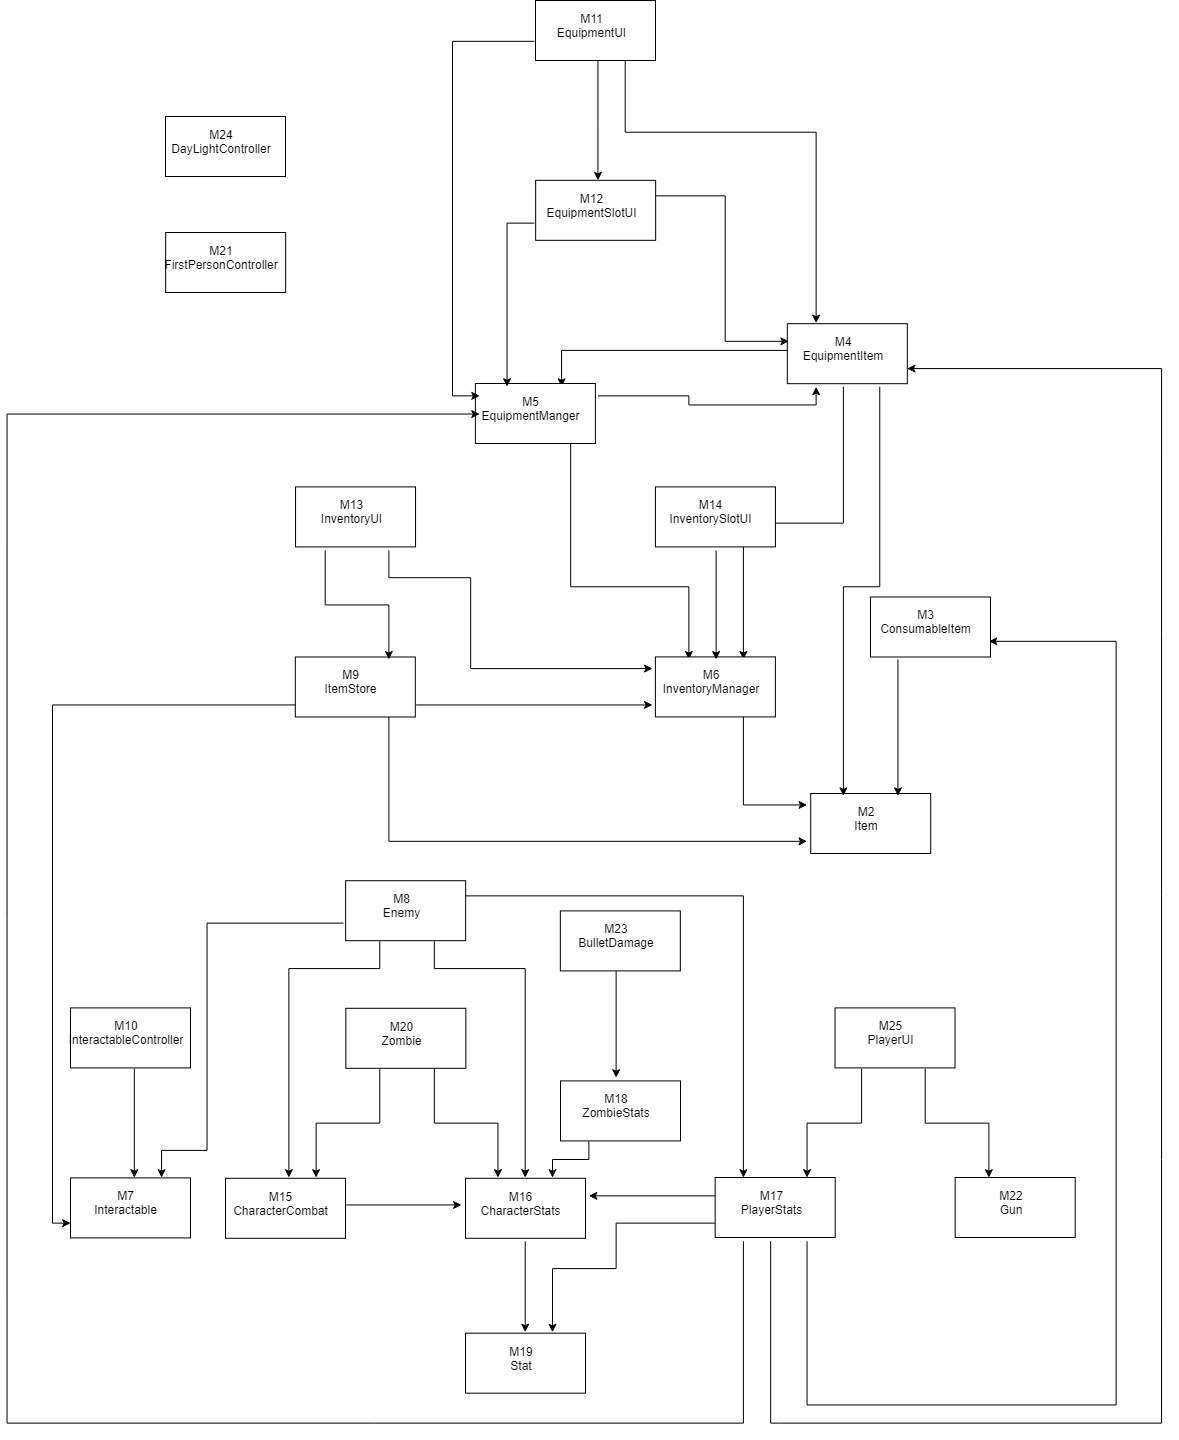
\includegraphics[scale=0.3]{UsesHierarchy.png}
\caption{Use hierarchy among modules}
\label{FigUH}
\end{figure}

\begin{table}[H]
\centering
\begin{tabular}{p{0.2\textwidth} p{0.6\textwidth}}
\toprule
\textbf{Modules} & \textbf{Uses}\\
\midrule
\mref{mHH} & ~\\
\mref{mSDI} & \mref{mHH}\\
\mref{mSDCI} & \mref{mSDIM}\\
\mref{mSDEI} & \mref{mSDEM}, \mref{mBHES}, \mref{mSDI}\\
\mref{mSDEM} & \mref{mSDIM}, \mref{mSDEI}\\
\mref{mSDIM} & \mref{mSDI}\\
\mref{mBHI} & ~\\
\mref{mBHE} & \mref{mBHCC}, \mref{mSDCS}, \mref{mSDPS}, \mref{mBHI}\\
\mref{mBHIS} & \mref{mSDI}, \mref{mBHI}, \mref{mSDIM}\\
\mref{mBHIC} & \mref{mBHI}\\
\mref{mBHEU} & \mref{mSDEM}, \mref{mBHES}\\
\mref{mBHES} & \mref{mSDEI}, \mref{mSDEM}\\
\mref{mBHIU} & \mref{mSDIM}, \mref{mBHIS}\\
\mref{mBHISU} & \mref{mSDIM}\\
\mref{mBHCC} & \mref{mSDCS}\\
\mref{mSDCS} & \mref{mSDS}\\
\mref{mSDPS} & \mref{mSDCS}, \mref{mSDS}, \mref{mSDEM}, \mref{mSDCI}, \mref{mSDEI}\\
\mref{mSDZS} & \mref{mSDCS}\\
\mref{mSDS} & ~\\
\mref{mBHZ} & \mref{mBHCC}, \mref{mSDCS}\\
\mref{mBHFPS} & ~\\
\mref{mBHG} & ~\\
\mref{mBHBD} & \mref{mSDCS}\\
\bottomrule
\end{tabular}
\caption{Use hierarchy among modules in table format for Figure \ref{FigUH}}
\label{TblACT}
\end{table}

%\section*{References}

\bibliographystyle {plainnat}
\bibliography {MG}

\end{document}